\documentclass[a4paper,10pt]{article}
\usepackage[utf8]{inputenc}
\usepackage{graphicx}
\usepackage{url}
\usepackage{float}
\usepackage{times}
\usepackage{multirow}
\usepackage{listings}
\usepackage{times}
\usepackage{paralist}
\usepackage{epsfig}
\usepackage{subfigure}
\usepackage[hypertex]{hyperref}
\usepackage{subfigure}
\usepackage{color}
\usepackage{xspace}

%\documentclass{rspublic}

\usepackage{ifpdf}

\newcommand{\I}[1]{\textit{#1}}
\newcommand{\B}[1]{\textbf{#1}}
\newcommand{\BI}[1]{\textbf{\textit{#1}}}
\newcommand{\T}[1]{\texttt{#1}}

\newcommand{\sagaspec}{\textit{SAGA}\xspace}
\newcommand{\sagaimpl}{\textit{SAGA}\xspace}

\newcommand{\spec}{\sagaspec}
\newcommand{\impl}{\sagaimpl}

\setlength\topmargin{0in}
\setlength\headheight{0in}
\setlength\headsep{0in}
\setlength\textheight{9.5in}
\setlength\textwidth{6.5in}
\setlength\oddsidemargin{0in}
\setlength\evensidemargin{0in}
\setlength\parindent{0.1in}
\setlength\parskip{0.25em}


\ifpdf
 \DeclareGraphicsExtensions{.pdf, .jpg,.jpeg}
\else
 \DeclareGraphicsExtensions{.eps, .ps}
\fi

\newcommand{\note}[1]{ {\textcolor{red} { ***NOTE: #1 }}}

\newif\ifdraft
\drafttrue

\ifdraft
\newcommand{\amnote}[1]{   {\textcolor{magenta} { ***Andre:    #1 }}}
\newcommand{\jhanote}[1]{  {\textcolor{red}     { ***Shantenu: #1 }}}
\else
\newcommand{\amnote}[1]{}
\newcommand{\jhanote}[1]{}
\fi

\begin{document}

 \title{ \Large \vspace{-3.5em} Mephisto Documentation }
 
 \author{ SAGA-Group}
 \date{05-04-2011}
 \maketitle
 

% \jhanote{Remember in addition to serving as an abstract, this will
%   serve as a summary of what will go to the 3 editors of the journals
%   that we are considering publishing a full paper in. Thus some more
%   information/discussion on what the underlying problem and context
%   will be about.}


% \jhanote{Once we have defined / introduced SAGA, we should probably
%   have 3 subsections -- interface, library and adatptors/backends?}

\section*{Introduction}
Mephisto is a perl script that supports SAGA (Simplified API for Grid Applications) 
installations. SAGA is an API that provides the basic functionality required to build 
distributed applications, tools and frameworks so as to be independent of the details 
of the underlying infrastructure ~\cite{saga-home} ~\cite{saga-tools}. More information
on SAGA can be found on the website:
\begin{verbatim}
  http://www.saga.cct.lsu.edu/
\end{verbatim}
SAGA installations require to install various dependency packages. 
Mephisto is a tool that automates the installation of SAGA, installing 
all its dependencies specified for SAGA and SAGA adaptors too.  
The version number of all the packages and the type of packages can 
be specified by the user at the command line. The description 
of all the command line options available are described 
in the next section.\\*
Example of the command line statement  
\begin{verbatim} perl mephisto install --target-dir=/home/user/saga --tmp-dir=/home/user/tmp-saga \end{verbatim}
Other examples with different command line options are explained in later section. \\*
\section*{Command line options}
This section discusses all the various options available at 
users disclosure. By default if no option is specified, mephisto 
pulls up the packages listed on the repositories
\begin{verbatim} 
http://static.saga.cct.lsu.edu/mephisto/repository/latest/INDEX. 
\end{verbatim}
Expanded version of the Command to run mephisto
\begin{verbatim} 
perl mephisto install/test --target-dir=/path/to/folder --tmp-dir=/path/to/folder 
--with-saga-version= --with-boost-version= --with-globus-version= 
--repository= --with-adaptors= --with-python-version= 
--with-postgresql-version=
\end{verbatim} 
\emph{install} \\*
 This can be used to install a working copy of SAGA and all its 
 dependencies specified. \\*
\emph{test} \\*
 This option not only installs SAGA but also runs the command 
 'make check' to check the installation. It creates a log file displaying 
 the test results. \\*
\emph{target-dir} \\*
 This option is used to specify the path you need to install SAGA and all 
 packages libraries. By default, it creates a folder at tmp/meph\_inst.\\*
\emph{tmp-dir} \\*
 This option is used to specify the path for a temporary folder to 
 download all the packages and create log files. By default, it 
 creates a folder at /tmp/meph\_tmp\\*
\emph{repository} \\*
 Can be used to choose different repositories to install SAGA from. 
 Two repositories available as of now are 'latest' (default) and svn\_trunk. 
 Recommended svn\_trunk for the most recent SAGA version. \\*
\emph{with-saga-version}\\*
 Choose saga versions available.\\*
\emph{with-boost-version}\\*
Choose boost versions available $>$=1.40.0\\*
\emph{with-globus-version} \\*
 Choose globus version available $>$=4.0. This option would automatically 
 invoke installations of X509, globus adaptors too. \\*
\emph{with-adaptors}\\*
 Mention any adaptors to install that would invoke globus installations along with 
 saga-adaptors too. \\*
 \emph{with-python-version}\\*
 Choose from the list of python versions available. Must be 
 $>$=2.6.2 \\*
 \emph{with-postgresql-version}\\*
 Choose from postgresql versions available. Should be $>$=8.4.1

\section*{Repositories for Mephisto} 
Mephisto uses two different repositories for SAGA packages which have been
pre-defined by the SAGA group, namely: 
\begin{verbatim}
(i) http://static.saga.cct.lsu.edu/mephisto/repository/latest/
\end{verbatim}
\begin{verbatim}
(ii) http://static.saga.cct.lsu.edu/mephisto/repository/svn_trunk
\end{verbatim}
When the user doesn't define any repository, the default 
repository taken by mephisto will be \emph {http://static.saga.cct.lsu.edu/
mephisto/repository/latest/}. \\*
The list of packages pre-defined for (i) are: \\*
SAGA= 1.5.2; \\*
Boost= 1.40.0; \\*
Python=2.6.2; \\*
Post-gre-sql=8.4 .1 ; \\*
Sqlite=3.6.18;   \\*
SAGA-PYTHON; \\*
SAGA-ADAPTORS-X509; \\*
SAGA-ADAPTORS-SSH.  \\*\\*
The list of packages pre-defined for (ii) are:
SAGA= 1.5.4 (updated as of now); \\*
Boost= 1.40.0; \\*
Python=2.6.2; \\*
Post-gre-sql=8.4 .1 ; \\*
Sqlite=3.6.18;   \\*
SAGA-PYTHON. \\*\\*
The suggested repository to be utilized by the user will be \emph{svn\_trunk} 
that is updated with the latest version of SAGA as and when
new version is released with bug fixes. Example to switch between 
repositories follows in the next section. 

\section*{Example Command line options}
\emph{NOTE: All examples here are tackled one at a time. They can be used interchangeably.
Choice has to be made between 'install' and 'test'}
\subsection*{- Basic Default command}
\begin{verbatim}
perl mephisto install 
\end{verbatim}
This would install SAGA. All the default options will be loaded as no
option was chosen here. As of now the default options are as foretold 
from the repository given below. As no directory was mentioned all the 
packages will be stored in a temporary folder created by the script.
\begin{verbatim}
http://static.saga.cct.lsu.edu/mephisto/repository/latest/
\end{verbatim}
%SAGA= 1.5.2;
%Boost= 1.40.0;
%Python=2.6.2;
%Post-gre-sql=8.4.1;
%Sqlite=3.6.18;
%SAGA-PYTHON;
%SAGA-ADAPTORS-X509;
%SAGA-ADAPTORS-SSH.

\subsection*{- Command with paths to folders}
\begin{verbatim}
perl mephisto install --target-dir=/path/to/any/desired-directory/ 
--tmp-dir=/path/to/temp/folder 
\end{verbatim}
This will install all packages in the folder specified. 
\subsection*{- Install SAGA from svn\_trunk repository}
\begin{verbatim}
perl mephisto install --target-dir=/path/to/any/desired-directory/ 
--tmp-dir=/path/to/temp/folder --repository=svn_trunk
\end{verbatim}
Choose snv\_trunk repository to install SAGA. This will have the most
recent and tested working SAGA version. 
\subsection*{- Install SAGA will all saga, globus, boost versions specified}
\begin{verbatim}
perl mephisto install --target-dir=/path/to/any/desired-directory/ 
--tmp-dir=/path/to/temp/folder --with-saga-version=1.5.3 
--with-boost-version=1.44.0 --with-globus-version=5.0.2
(or)
perl mephisto install --target-dir=/path/to/any/desired-directory/ 
--tmp-dir=/path/to/temp/folder --with-saga=1.5.3 
--with-boost=1.44 --with-globus=5.0.2
\end{verbatim}
To install SAGA with different boost, SAGA and globus versions.
Given here are two ways of defining the versions. Using all the three 
is not compulsory and any combination can be used. Any version 
not mentioned will infer default options. 
\subsection*{- Globus installations}
\begin{verbatim}
perl mephisto install --target-dir=/path/to/any/desired-directory/ 
--tmp-dir=/path/to/temp/folder --with-globus-version=5.0.2
\end{verbatim}
Specifying any globus installations will also invoke globus adaptors
installations which are required and necessary with globus.
\subsection*{- Install SAGA with Globus adaptors}
\begin{verbatim}
perl mephisto install --target-dir=/path/to/any/desired-directory/ 
--tmp-dir=/path/to/temp/folder --with-adaptors=globus
\end{verbatim}
To install globus adaptors. Automatically invokes globus installations which 
is required for adaptors. Also automates x509 adaptors installations too.
This is similar to what we have in the previous example but different 
command line options have been given for easy usage.  
\subsection*{- How to install a SAGA Core Pre-Release with a specific Boost version (for developers)}
\begin{verbatim}
perl mephisto install --target-dir=/path/to/any/desired-directory/ 
--tmp-dir=/path/to/temp/folder --with-saga=1.5.3-pre
\end{verbatim}
For developers, this would install the pre-release version from the given 
link shared in the email with boost and all other dependencies creating log 
files necessary for debugging. 
\subsection*{- Install with Python versions}
\begin{verbatim}
perl mephisto test --target-dir=/path/to/any/desired-directory/ 
--tmp-dir=/path/to/temp/folder --with-python-version=2.7.1
\end{verbatim}
Install with any python version $>$=2.6.2. Please note that you may 
be thrown an error and break from the build for versions incompatibility.
\subsection*{- Install with postgresql version}
\begin{verbatim}
perl mephisto test --target-dir=/path/to/any/desired-directory/ 
--tmp-dir=/path/to/temp/folder --with-postgresql-version=8.4.2
\end{verbatim}
Similar to what was described earlier for python versions right above.
\subsection*{- Install and proceed to TEST the installations}
\begin{verbatim}
perl mephisto test --target-dir=/path/to/any/desired-directory/ 
--tmp-dir=/path/to/temp/folder --with-saga-version=1.5.3 
--with-boost-version=1.44.0 --with-globus-version=5.0.2
\end{verbatim}
Choose 'test' option to first install SAGA and its dependencies and then have it
continuously perform 'make check' operation and create a log file in the end.
\section*{Example of a Screen Shot after execution}
\subsection*{- User command options screen}
\begin{figure}[H]
\begin{center}
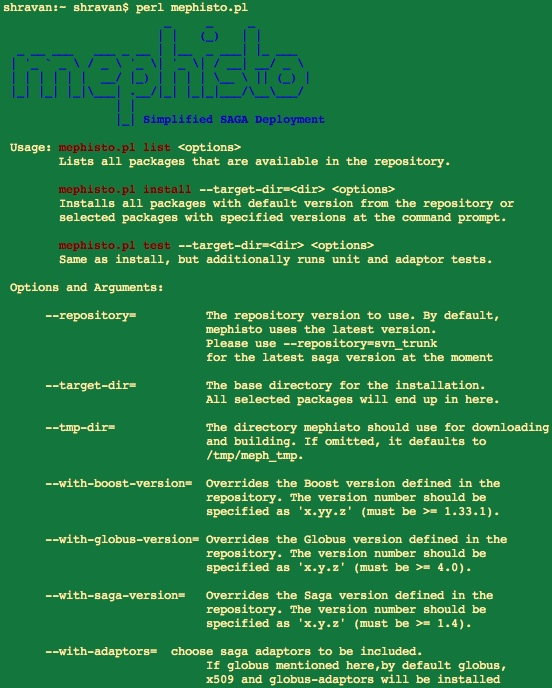
\includegraphics[scale=0.60]{userscreen1.jpg}
\end{center}
\end{figure}
\subsection*{- svn\_trunk repository used}
\begin{figure}[H]
\begin{center}
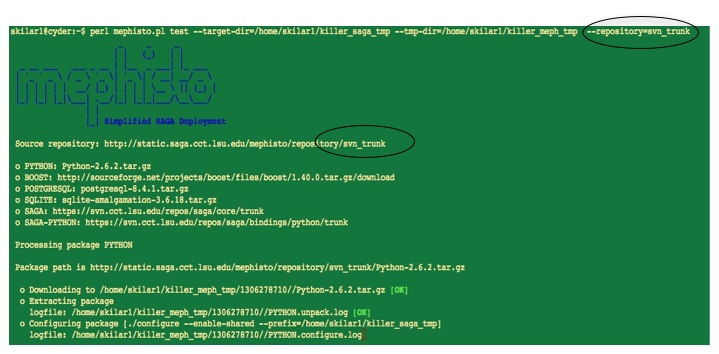
\includegraphics[scale=0.60]{svntrunk.jpg}
\end{center}
\end{figure}
\subsection*{- latest repository used (default)}
\begin{figure}[H]
\begin{center}
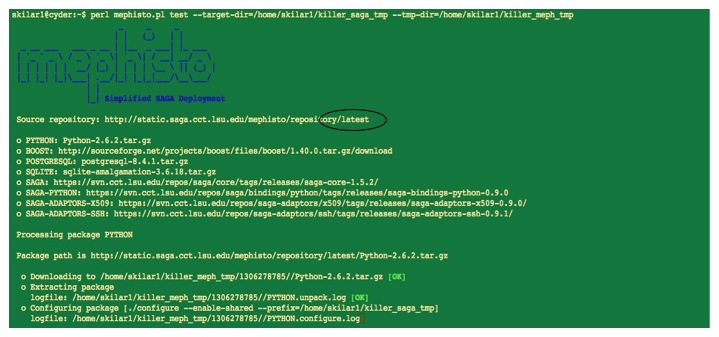
\includegraphics[scale=0.60]{latest.jpg}
\end{center}
\end{figure}
\subsection*{- Successful installations done}
\begin{figure}[H]
\begin{center}
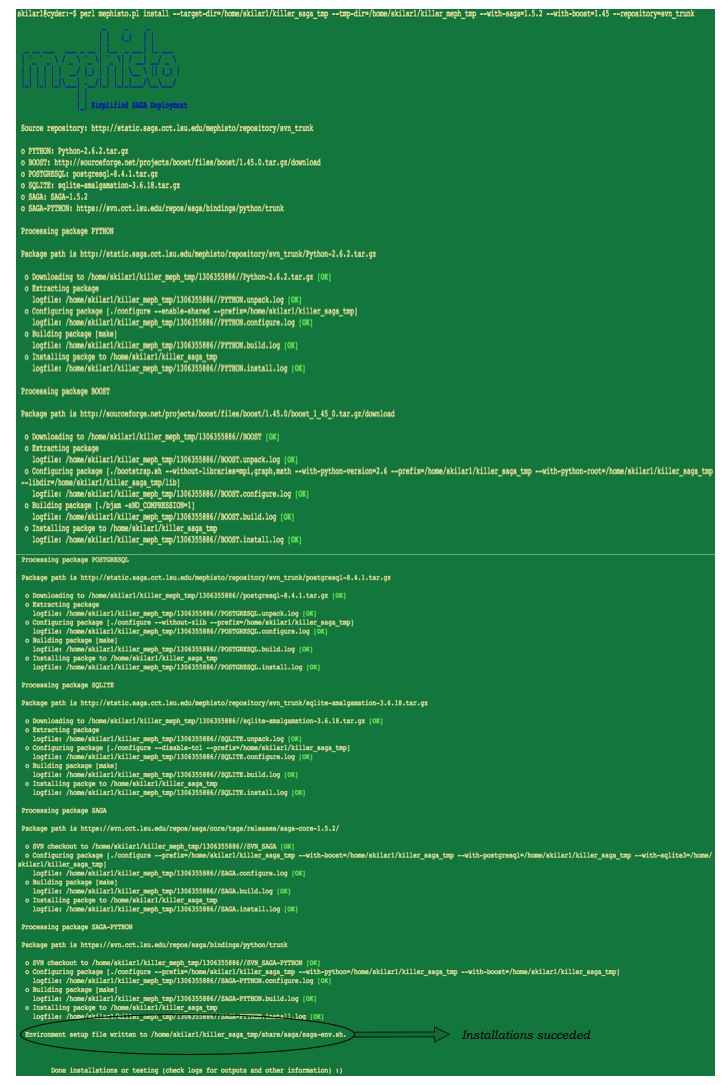
\includegraphics[scale=0.60]{install_succ.jpg}
\end{center}
\end{figure}
\subsection*{- Successful Testing done}
\begin{figure}[H]
\begin{center}
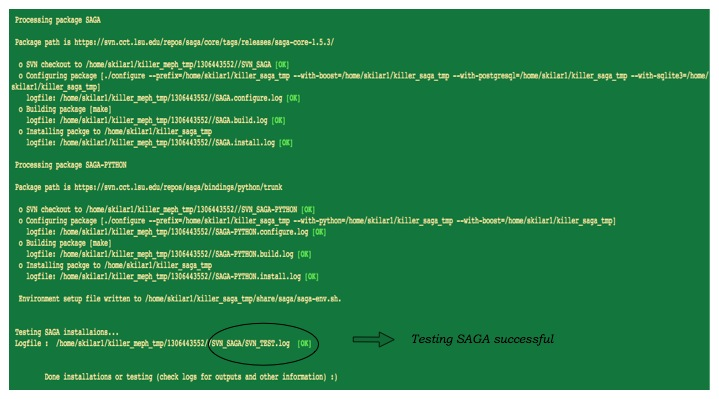
\includegraphics[scale=0.60]{test_succ}
\end{center}
\end{figure}
\subsection*{- Installation failed}
\begin{figure}[H]
\begin{center}
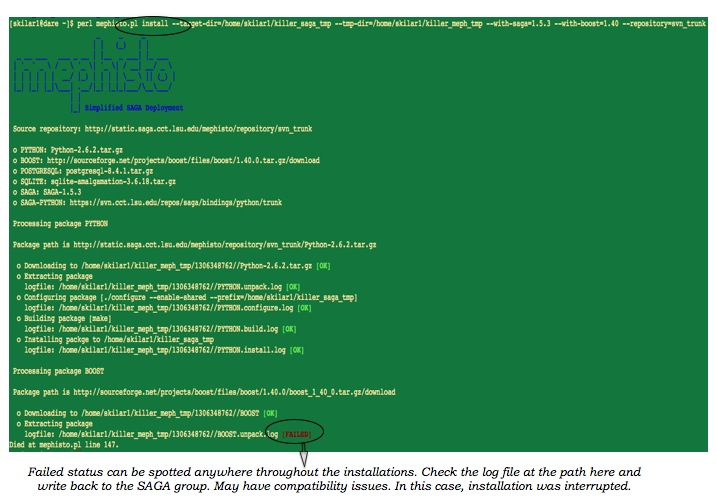
\includegraphics[scale=0.60]{install_fail.jpg}
\end{center}
\end{figure}
\subsection*{- Testing failed}
\begin{figure}[H]
\begin{center}
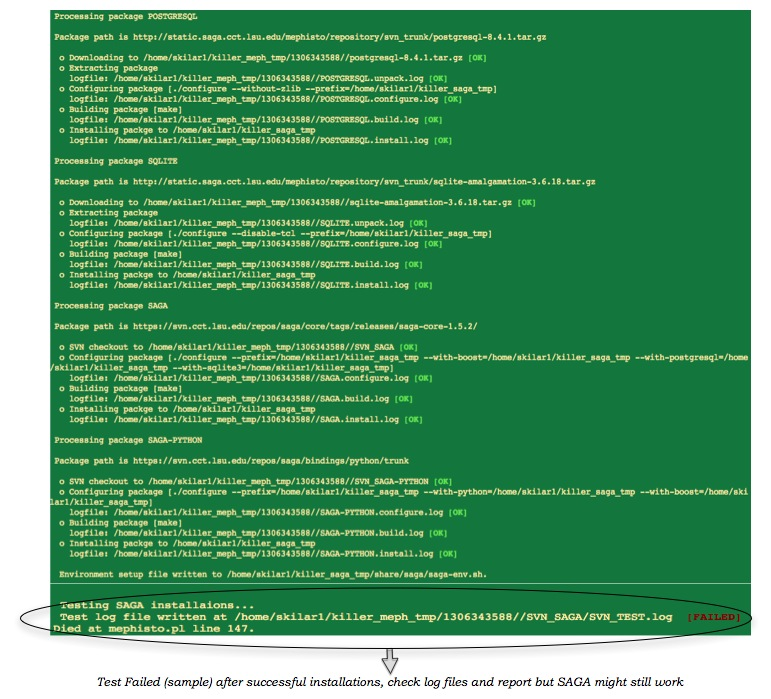
\includegraphics[scale=0.60]{test_fail.jpg}
\end{center}
\end{figure}
%\begin{figure}
%\begin{center}
%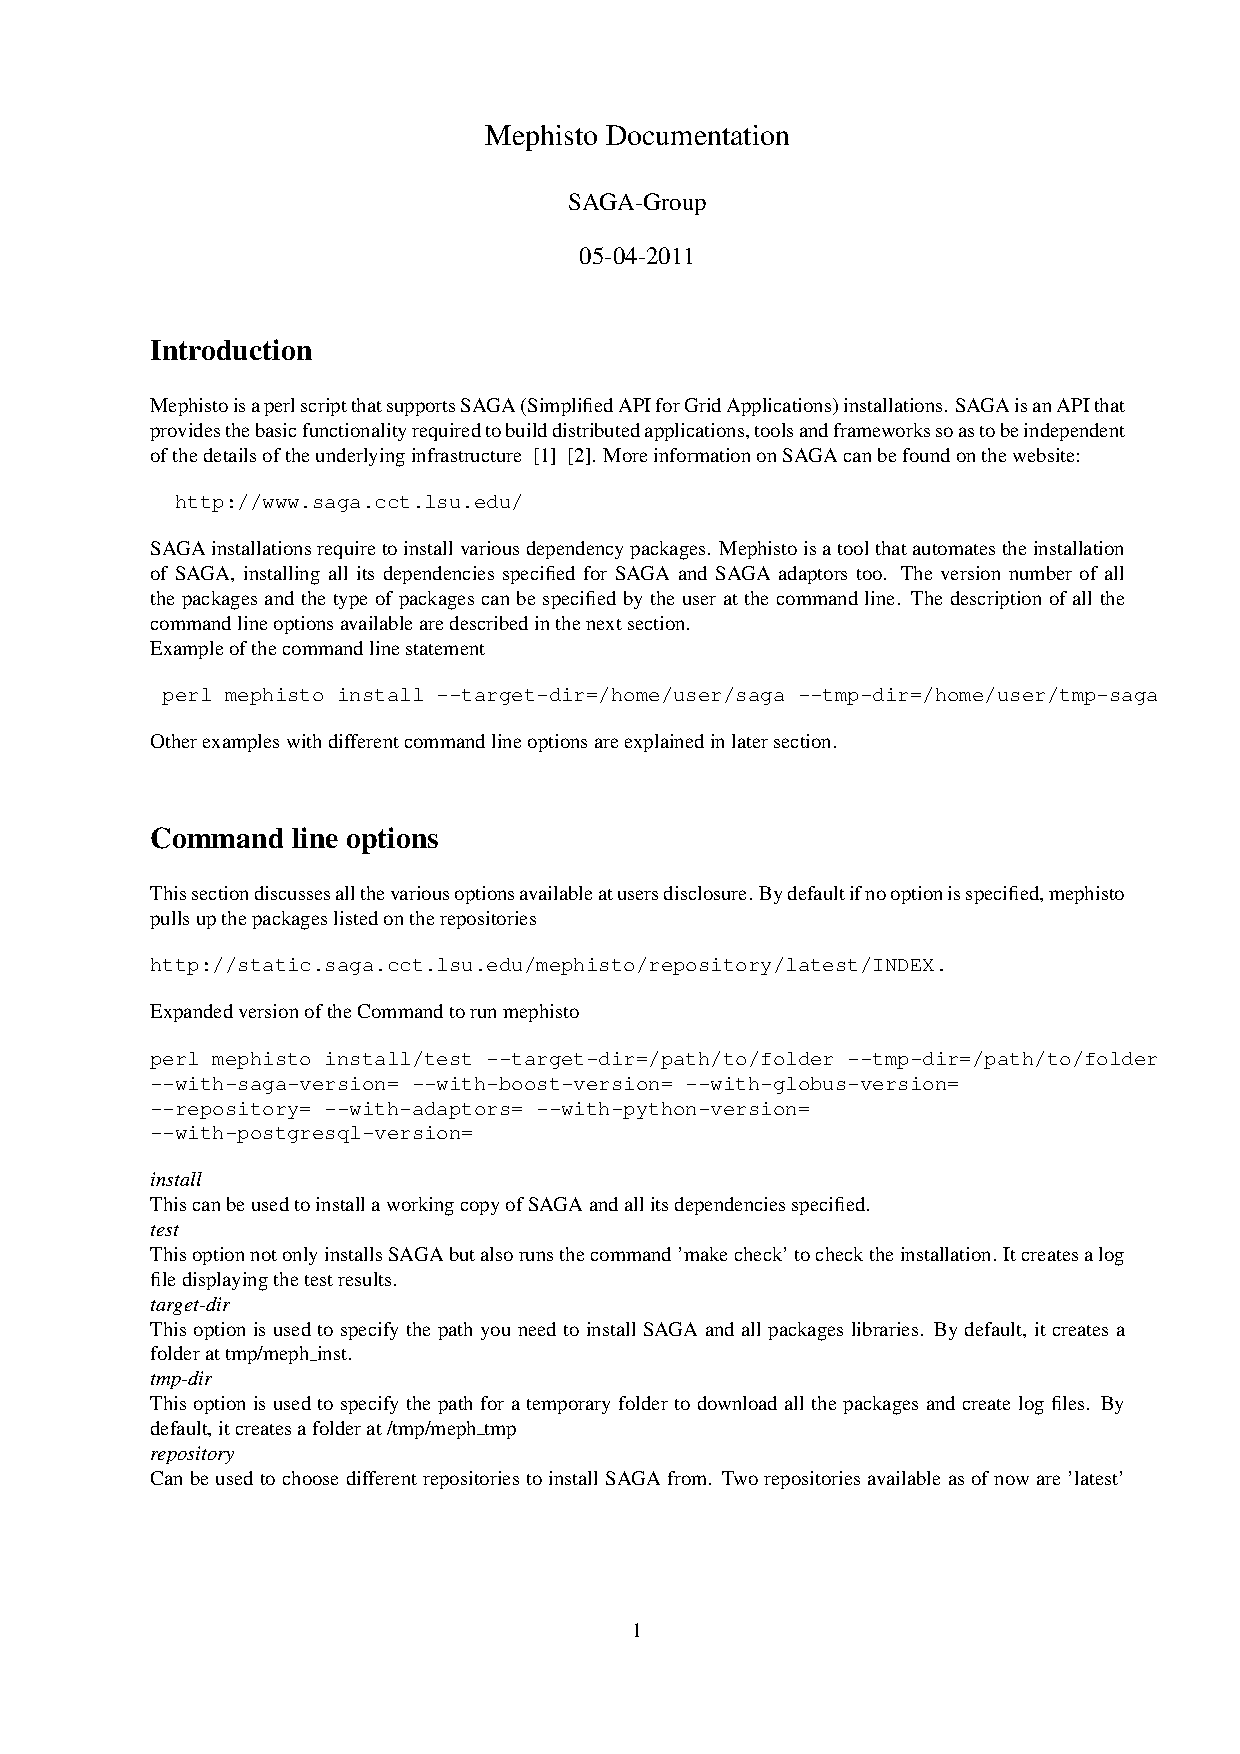
\includegraphics[scale=0.60]{mephistodocumentation.jpg}
%\end{center}
%\caption{The programming abstractions provided by the AllPairs and
%  MapReduce algorithm implementations are sufficient to enable a wide
%  range of genomic applications (sequence alignment, searching, etc.)
%  to be distributed over grids. The required underlying functionality
%  is provided by higher level algorithmic support abstractions, such
%  as tools for data placement, latency hiding, and job distribution,
%  which are being built on top of grid middleware abstractions
%  provided by SAGA (such as file transfer, job launching, information
%  services and replica management.}
%\label{fig:mephistodocumentation}
%\end{figure}
\section*{Possible errors and debugging} 
Mephisto throws in an error saying "Failure" at the step it failed to execute. 
It dies with no further operation. The installation is halted with packages stored 
in the directory mentioned at the command line or default directory (if not mentioned).
Note that the installation doesn't start where it halted. Log files are available and the
path to the file is displayed on the screen for access and assessment. 
Possible errors and actions: \\*
1) Version incompatibility: Any version incompatibility issues seen in the 
log files should be reported to saga-users@cct.lsu.edu and/or 
saga-devel@cct.lsu.edu mailing lists with the log files attached. 
Proper package compatible versions will be suggested or necessary changes 
will be made to SAGA package.\\*
2) Failure to download package: This can be a serious bug in the mephisto code which means 
that the link is broken and necessary changes have to be made in order to have the version
taken. Reporting to the above mailing lists will do the trick. Sometimes there are server
problems from the website its downloading. Have few trials done with some time
lapse between each run before confirming the error. \\*
3) Wrong Directory Sorted(as seen in the log file) : This will mean a bug in the perl script 
and should be reported in the similar manner. People working on mephisto will get it fixed. 
Shouldn't be a problem and was not found till date. \\*

 
 \bibliographystyle{IEEEtran} 
 \bibliography{mephisto}


\end{document}

